\chapter{ARACNE-structure learning}
\label{ch-aracne}

This chapter
is based on
Ref.\cite{aracne}.


The ARACNE algo
considers data samples
for $n$ random variables
$(x_i)_{i=0, 1, \dots, n-1}$.
and estimates the mutual
information $MI_{i,j}=H(\rvx_i:\rvx_j)$ between
every pair of nodes.
The algo 
starts with a fully connected
undirected graph $UG$.
Next the algo
removes from $UG$
every edge with $MI_{i,j}<\eps$
for some threshold $0<\eps<<1$.
Then the algo examines every
triplet of nodes and marks for removal 
the edge of the triplet
with the smallest MI.
Finally,
the algo removes from $UG$  all
edges marked for removal.
 Each triplet is analyzed
irrespective of whether its edges
 have been marked for
removal when considering a prior triplet.
Thus the network constructed by the 
algorithm is independent of the
 order in which the triplets are examined.

Ref.\cite{aracne} incorrectly claims that
removing the smaller of 3 MI's
is motivated by the Data Processing 
Inequality (DPI)
of Shannon Information Theory. 
See Chapter \ref{ch-mchain}
for more info about DPI.
Note that DPI is
only valid for a Markov chain,
and not all
 triplets of random variables
are in a Markov chain.
Motivating the removal of the smaller of 
3 numbers does not require DPI.

\begin{figure}[h!]
\centering
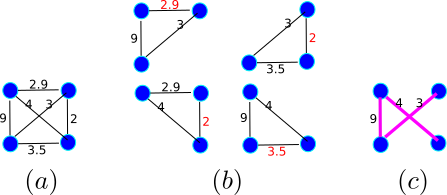
\includegraphics[width=4in]
{aracne/aracne.png}
\caption{
Example of ARACNE that gives Chow-Liu tree.
$(a)$ Fully connected 
undirected graph with
 weights $MI_{i,j}$
along the edges.
$(b)$ All 4 possible triplets of nodes.
Edges marked for removal 
have their weights
printed in red.$(c)$
Final structure.} 
\label{fig-aracne}
\end{figure}


Fig.\ref{fig-aracne}
gives an example 
of the application
of the ARACNE algo.

See Chapter \ref{ch-chow} on 
the Chow-Liu trees (CLT).
A CLT is just
a  maximum spanning tree
where the weights are 
mutual informations 
 $MI_{i,j}$
estimated from data.

Sometimes, the outcome
of the ARACNE algo is a CLT.
For example,
Fig.\ref{fig-aracne}
$(a)$
was considered
in Chapter \ref{ch-chow}
on CLTs, where
the CLT algo
also
gave 
Fig.\ref{fig-aracne}
$(c)$ as the final structure.

According to Ref.\cite{aracne}, the 
 ARACNE algo sometimes 
yields a structure with loops.
Hence, it does not always yield a CLT,
or even a tree, or even a polytree (i.e., 
a connected bnet with no loops).


